%%%%%%%%%%%%%%%%%%%%%%%%%%%%%%%%%%%%%%%%%
% "ModernCV" CV and Cover Letter
% LaTeX Template
% Version 1.1 (9/12/12)
%
% This template has been downloaded from:
% http://www.LaTeXTemplates.com
%
% Original author:
% Xavier Danaux (xdanaux@gmail.com)
%
% License:
% CC BY-NC-SA 3.0 (http://creativecommons.org/licenses/by-nc-sa/3.0/)
%
% Important note:
% This template requires the moderncv.cls and .sty files to be in the same 
% directory as this .tex file. These files provide the resume style and themes 
% used for structuring the document.
%
%%%%%%%%%%%%%%%%%%%%%%%%%%%%%%%%%%%%%%%%%

%----------------------------------------------------------------------------------------
%	PACKAGES AND OTHER DOCUMENT CONFIGURATIONS
%----------------------------------------------------------------------------------------

\documentclass[11pt,a4paper,sans]{moderncv} % Font sizes: 10, 11, or 12; paper sizes: a4paper, letterpaper, a5paper, legalpaper, executivepaper or landscape; font families: sans or roman

\moderncvstyle{classic} % CV theme - options include: 'casual' (default), 'classic', 'oldstyle' and 'banking'
\moderncvcolor{blue} % CV color - options include: 'blue' (default), 'orange', 'green', 'red', 'purple', 'grey' and 'black'

\usepackage[scale=0.93]{geometry} % Reduce document margins
\usepackage[utf8]{inputenc}
\usepackage{pgfplots}

\definecolor{s1}{RGB}{56,115,179}
\renewcommand*{\namefont}{\fontsize{24}{29}\mdseries\upshape}
%\setlength{\hintscolumnwidth}{3cm} % Uncomment to change the width of the dates column
%\setlength{\makecvtitlenamewidth}{10cm} % For the 'classic' style, uncomment to adjust the width of the space allocated to your name
\usepackage{xpatch}% http://ctan.org/pkg/xpatch
\xpatchcmd{\cvitem}{#3}{\footnotesize #3}{}{}

%----------------------------------------------------------------------------------------
%	NAME AND CONTACT INFORMATION SECTION
%----------------------------------------------------------------------------------------

\firstname{Pierre} % Your first name
\familyname{Rouveyrol} % Your last name

% All information in this block is optional, comment out any lines you don't need
%\title{Curriculum Vitae}
\address{29T, Avenue Pasteur}{74100 Annemasse, France}
\mobile{+336 34 16 24 34}
%\phone{04 56 33 40 20}
%\fax{(000) 111 1113}
\email{pierre.rouveyrol@protonmail.com}
\homepage{https://gitlab.com/Oakenston}{https://gitlab.com/Oakenston} % The first argument is the url for the clickable link, the second argument is the url displayed in the template - this allows special characters to be displayed such as the tilde in this example
\extrainfo{Nationality : Swiss, French}
%\photo[50pt][0pt]{pictures/portrait} % The first bracket is the picture height, the second is the thickness of the frame around the picture (0pt for no frame)
\quote{IT Management, Infosec, Devops, Open Source, 5 years experience}

\renewcommand*\namefont{\fontsize{25}{48}\selectfont}
\renewcommand*\sectionfont{\fontsize{14}{24}\selectfont}
\renewcommand*\subsectionfont{\fontsize{11}{24}\selectfont}
\renewcommand*\hintfont{\fontsize{10}{24}\selectfont}
\pgfplotsset{compat=1.15}

%----------------------------------------------------------------------------------------

\begin{document}

\makecvtitle % Print the CV title

%----------------------------------------------------------------------------------------
%	EDUCATION SECTION
%----------------------------------------------------------------------------------------

\section{Education}
\subsection{Academic}
\cventry{2015-2016}{Master 2 cybersecurity}{SAFE}{Université Joseph Fourier}{}{}
\cventry{2013-2014}{Master 1 computer science}{International program, MoSIG}{Université Joseph Fourier}{}{}
\cventry{2012-2013}{Bachelor computer science}{Video games conception}{Université du Québec à Chicoutimi}{}{}
\cventry{2010-2012}{DUT Informatique (French 2 year diploma)}{IUT 2 de Grenoble}{Université Pierre Mendès-France}{\textit{Rank : 10/84}}{}
\cventry{2007-2010}{Baccalauréat S-SI (Engineering)}{Lycée Ferdinand Buisson}{}{}{}

\subsection{MOOC}
\cventry{Jul-Sep 2013}{Computer Networks}{https://www.coursera.org/}{Washington university's networks course}{\textit{Grade : 96/100}}{}
\cventry{Oct-Déc 2011}{AI-Class}{https://www.ai-class.com/}{Stanford's introductory Artificial Intelligence course}{\textit{Grade : 98/100}}{}

%----------------------------------------------------------------------------------------
%	COMPUTER SKILLS SECTION
%----------------------------------------------------------------------------------------
\section{Skills}
\centering
\pgfplotsset{height=3cm,width=9cm}
\pgfplotsset{xticklabel style={text width=4.8em,align=right}}
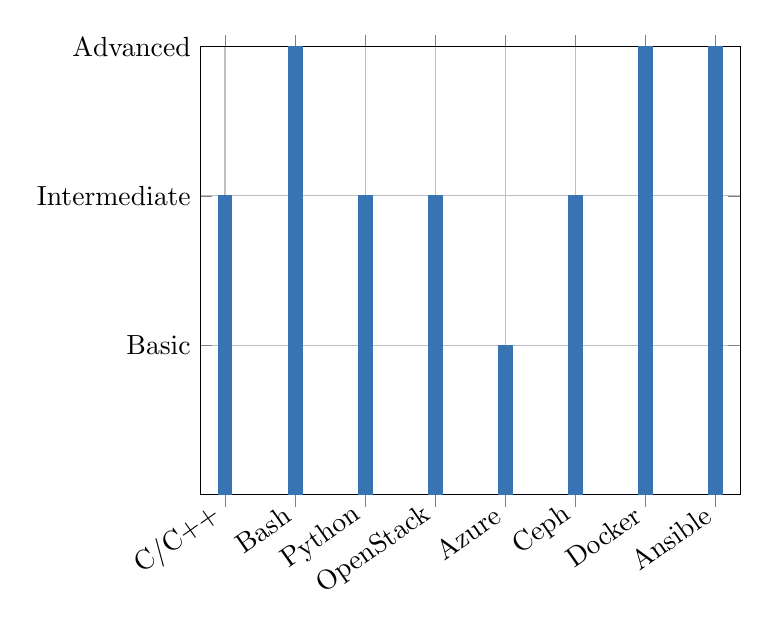
\begin{tikzpicture}
	\begin{axis}[ybar,
			enlarge y limits=0,
			enlarge x limits=0.05,
			legend style={at={(0.5,-0.2)}, anchor=North, legend columns=-1},
			symbolic x coords={ C/C++, Bash, Python, OpenStack, Azure, Ceph, Docker, Ansible},
			symbolic y coords={ X, Basic, Intermediate, Advanced},
			ymax=Advanced,
			ymin=X,
			ytick=data,
			xtick=data, 
			grid=both,
			x tick label style={rotate=35,anchor=east},
			bar width = 5pt]

		\addplot [fill=s1,draw=s1] coordinates {(C/C++,Intermediate)(Bash,Advanced)(Python,Intermediate)(OpenStack,Intermediate)(Azure,Basic)(Ceph,Intermediate)(Docker,Advanced)(Ansible,Advanced)};
	\end{axis}
\end{tikzpicture}
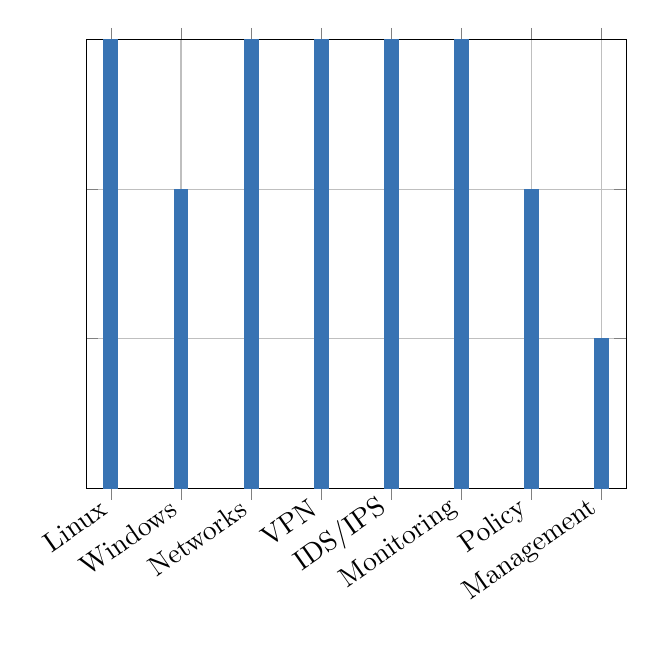
\begin{tikzpicture}
	\begin{axis}[ybar,
			enlarge y limits=0,
			enlarge x limits=0.05,
			legend style={at={(0.5,-0.2)}, anchor=North, legend columns=-1},
			symbolic x coords={Linux, Windows, Networks, VPN, IDS/IPS, Monitoring, Policy, Management},
			symbolic y coords={ X, Basic, Intermediate, Advanced},
			ymax=Advanced,
			ymin=X,
			ytick=data,
			yticklabels={,,},
			xtick=data, 
			grid=both,
			x tick label style={rotate=35,anchor=east},
			bar width = 5pt]	
		\addplot [fill=s1,draw=s1] coordinates {(Linux,Advanced)(Windows,Intermediate)(Networks,Advanced)(VPN,Advanced)(IDS/IPS,Advanced)(Monitoring,Advanced)(Policy,Intermediate)(Management,Basic)};
	\end{axis}
\end{tikzpicture}

%----------------------------------------------------------------------------------------
%	LANGUAGES SECTION
%----------------------------------------------------------------------------------------

\section{Languages}
\cvitemwithcomment{French}{Native}{}
\cvitemwithcomment{English}{Fluent}{Numerous travels abroad (Irland, UK, US, Canada...) and all work in English}
\cvitemwithcomment{German}{Basic}{3 years in school}

%----------------------------------------------------------------------------------------
%	WORK EXPERIENCE SECTION
%----------------------------------------------------------------------------------------
\section{Experience}

\cventry{2021-2022}{Systems and Automation Engineer}{\textsc{Infomaniak}}{Geneva}{}{Part of the team in charge of infrastructure maintenance and improvement. \newline Night and weekend shifts.}
\cventry{2020-2021}{IT Security Specialist}{\textsc{MSC}}{Geneva}{}{Second in charge of headquarters security, preparations for migration of infrastructure to Azure. \newline Deployment and management of worldwide whitelisting policy. \newline Worldwide level 3 support on security related matters.}
\cventry{2017-2020}{IT Security Specialist}{\textsc{Viseo Group}}{Grenoble}{}{In charge of company wide security improvement, maintenance and incident response. \newline International level 3 IT support for Linux systems, networks and cloud infrastructure. \newline Design, implementation and maintenance of monitoring and SIEM systems.}
\cventry{2015-2016}{Cybersecurity Engineer}{\textsc{Thales}}{Montbonnot}{13 Months}{Security consulting on an undisclosed SCADA project.}
\cventry{2014-2015}{Research Engineer}{\textsc{Inria : Privatics}}{Montbonnot}{10 Months}{Research and development of a password guessing algorithm for targeted attacks. \newline Several talks given about the project and its targets and implications.}
\cventry{Mar-Sept 2014}{Research Intern}{\textsc{Inria : Privatics}}{Montbonnot}{6 Months}{Feasibility assessment of consumer grade Wi-Fi APs exploitation as a geotracking botnet.}
%\cventry{May-June 2012}{Academic internship}{\textsc{Groupe Folder}}{Voiron}{2 Months}{Debugging and updating of a client support website in .NET.}
%\cventry{November 2012}{Hackfest}{}{Québec}{}{Participation to the CTF : http://www.hackfest.ca/en/hacking-games/friday}
%\cventry{June 2013}{Nuits du Hack}{}{Paris}{}{Participation to OVHack and a lockpicking challenge}
%\vspace{1mm}
%\cventry{Summers}{Carpentery, EDF meters survey, Mail sorting, Gardening}{}{}{}{}
%\cventry{Events}{Attended and gave talks, some CTF and lockpicking challenges}{}{}{}{}

%----------------------------------------------------------------------------------------
%	INTERESTS SECTION
%----------------------------------------------------------------------------------------
%\section{Interests}

%\renewcommand{\listitemsymbol}{-~} % Changes the symbol used for lists

%\cvlistdoubleitem{Mountain sports : Paragliding, ski, hiking}{Motorcycle}
%\cvlistdoubleitem{Crafting : Blacksmithing, Electronics, DIY}{Corporate security (Tech \& Social)}
%\cvlistdoubleitem{Permaculture}{Precision Shooting}
%----------------------------------------------------------------------------------------

\end{document}
